%%%%%%%%%%%%%%%%%%%%%%%%%%%%%%%%%%%%%%%%%%%%%%%%%%%%%%%%%%%%%%%%%%%%%%%%%%
%%%%%%%%%%%%   CAPTER 3   %%%%%%%%%%%%%%%%%%%%%%%%%%%%%%%%%%%%%%%%%%%%%%%%
%%%%%%%%%%%%%%%%%%%%%%%%%%%%%%%%%%%%%%%%%%%%%%%%%%%%%%%%%%%%%%%%%%%%%%%%%%
\chapter{Existing Analysis}
\label{chap:existing_analysis}
The Radar processor should be capable of processing both the Air to Air mode data as well as Air to Ground mode data (SAR). Scope of this thesis is limited to A/A Mode processing. Mode mapping analysis in this chapter are based on the timing information provided in the Table \ref{tbl:aa_exe}. Existing work by Airbus DS\cite{fcas} configures the mode mapping in accordance to Space Partition and Time Partition.\\ 

\noindent
\textbf{Time Partitioning:}\\
One iMX6Quad CPU is time sliced to run A/A mode and A/G mode alternatively. The timeframe between two subsequent A/A mode execution is called major time frame. Memory and cache are also partitioned for each mode. Intra-partition communication can be done by buffers, semaphores and/or events. When the time slice is completed for Air to Air mode, context switch happens to store the details of A/A Mode and load the details of A/G Mode, afterwards the A/G mode begins execution. Violation of timing behaviour triggers an exception. \\

\noindent
\textbf{Space Partitioning:} \\
A/A mode processing and A/G mode processing are done in separate physical entities. It is the simplest configuration for dedicated data processing. Failure of one of the systems will not affect the other as they are independent. It is assumed that SDRAM and L2 cache are partitioned for 4 cores to improve determinism. Each core has pre-defined accessible address space in Memory and L2 cache. 

%%%%%%%%%%%%%%%%%%%%%%%%%%%%%%%%%%%%%
%%%%%%%%%%%%%%%%%%%%%%%%%%%%%%%%%%%%%
%%%%%%%%%%%%   SECTION   %%%%%%%%%%%%
%%%%%%%%%%%%%%%%%%%%%%%%%%%%%%%%%%%%%
%%%%%%%%%%%%%%%%%%%%%%%%%%%%%%%%%%%%%
\section{Scheme 1 - Space Partitioning}
\label{sec:scheme_1}
This section explains the formulas and calculations in the excel document provided by Airbus DS. A RADAR echo received by the Radar antenna is distinguished as A/A mode or A/G mode by the iCON1 module.

\begin{figure}[h!]
	\centering
	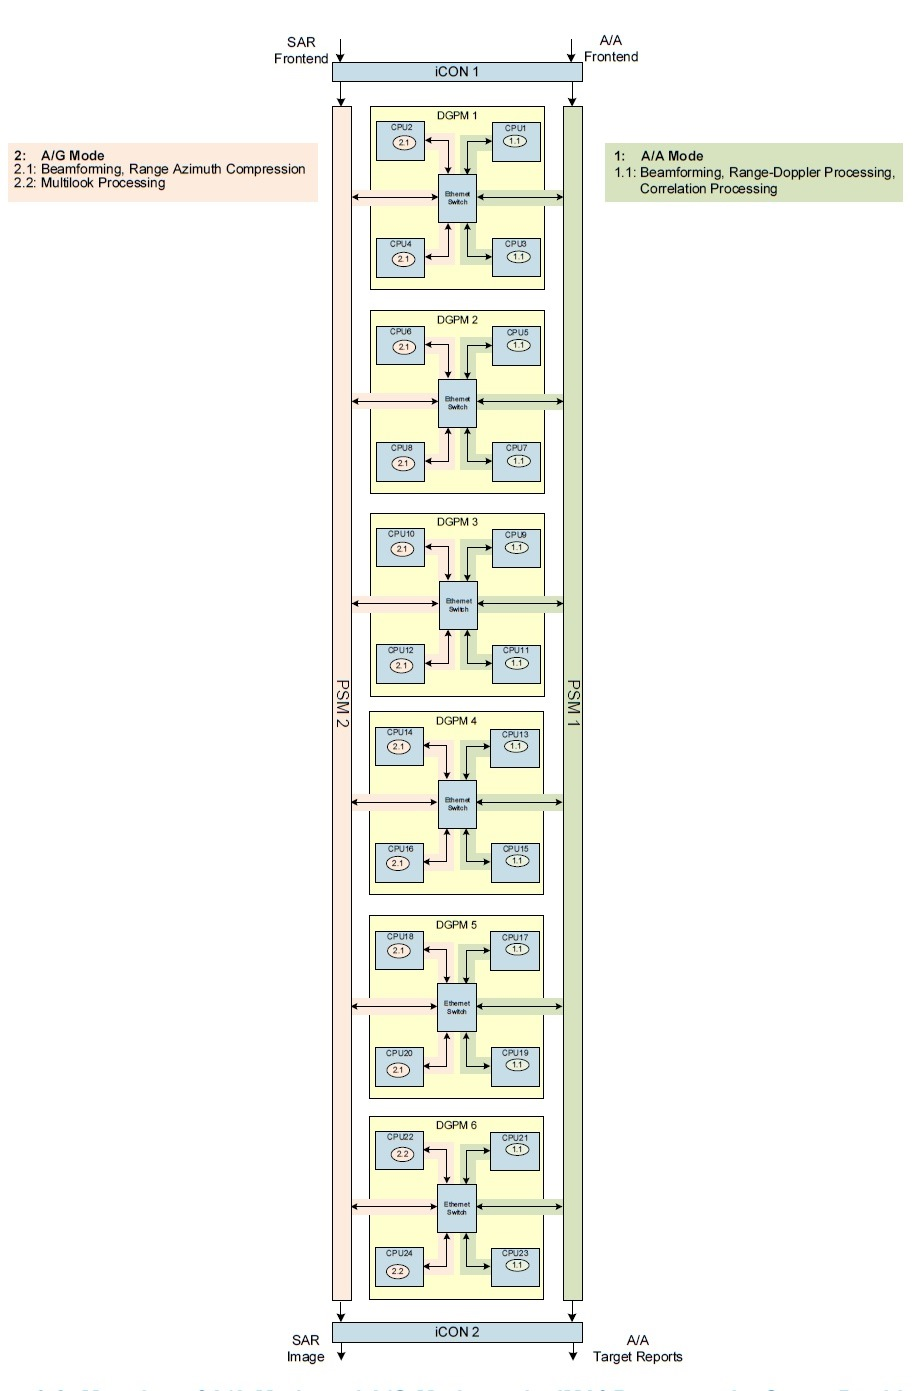
\includegraphics[width=160mm, height=220mm]{figures/scheme1}
	\caption{ Scheme-1, Mode Mapping}
	\label{fig:existing_analysis:scheme1}
\end{figure}
\FloatBarrier

A/A mode data are redirected to PSM1 and A/G mode data are sent to PSM2. The two odd numbered CPUs(CPU1 and CPU3) of a  DGPM are allocated to the processing of the A/A mode. The two even numbered CPUs(CPU2 and CPU4)  of a DPGM are alloctated to the processing of the A/G mode. Each CPU with it's 4 cores is completely used for either A/A Mode or A/G mode processing.

\begin{tabular}{rl}
	Number of DGPMs: & 6 \\
	Number of CPUs: & 6 x 4 = 24 \\
	CPUs for A/A Mode: & 12 \\
	CPUs for A/G Mode: & 12 \\
\end{tabular}

\noindent
DGPM sends the processed data to iCON2 via respective PSM. iCON2 redirects A/A data to the Tracking processor and A/G data to the Display processor. The SDRAM is assumed to be partitioned for all the four cores, where every core has its buffer memory intended to transfer data between the cores and storage memory to store the data for Radar processing.

%%%%%%%%%%%%%%%%%%%%%%%%%
%%%%%   SUB-SECTION   %%%
%%%%%%%%%%%%%%%%%%%%%%%%%
%%%%%%%%%%%%%%%%%%%%%%%%%
\subsection{A/A Mode Results}
\label{ss:scheme1:aa}
Each CPU processes a dwell of data. The processing results are dispatched to iCON2 by PSM1. As the dwell data processing is independent to the processing of the predecessor dwell data and indepentent to the processing of the successor dwell data, there  is no data dependency between CPUs processing different dwell data.

\begin{figure}[h!]
	\centering
	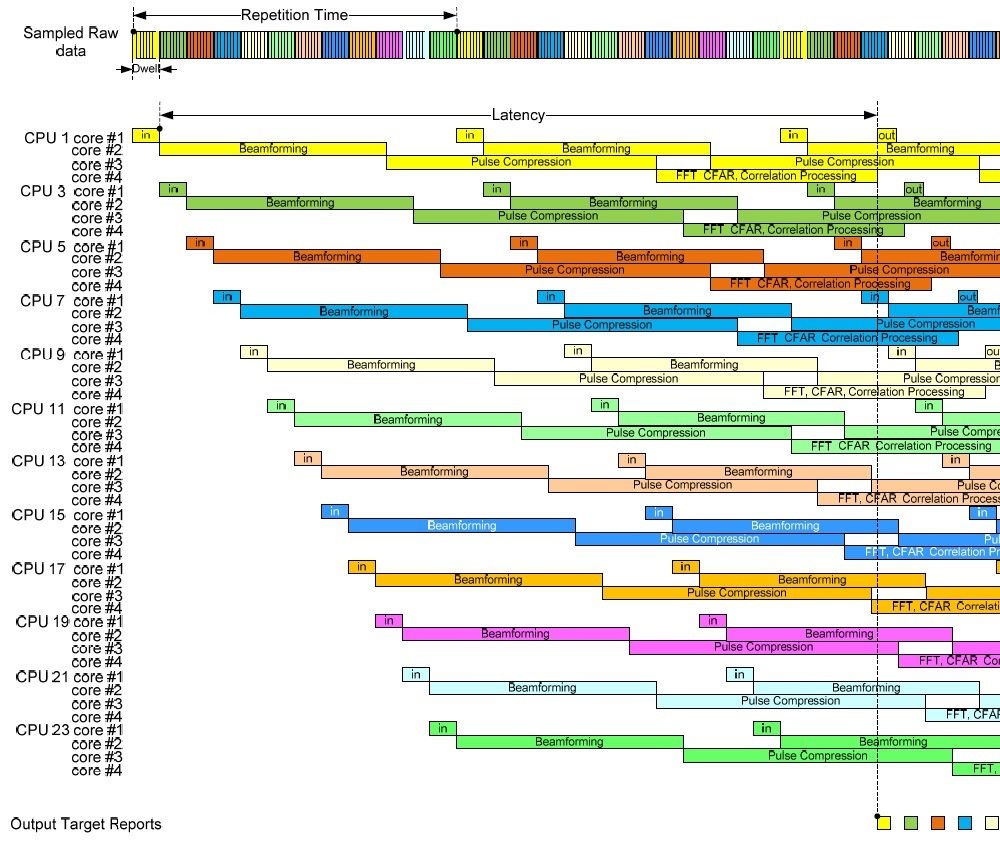
\includegraphics[width=140mm]{figures/aa_scheme1}
	\caption{Scheme-1, A/A Mode Processing}
	\label{fig:existing_analysis:aa_scheme1}
\end{figure}

%%%%%%%%%%%%%%%%%%%%%%%%%
%%%%%  SSUB-SECTION   %%%
%%%%%%%%%%%%%%%%%%%%%%%%%
\subsubsection{CPU Utilization}
\label{sss:scheme1:aa:cpu_util}
CPU utilization is the ratio of processing time to the available time. The worst case available time of a CPU is the time span between receiving two shortest dwells by the CPU, calculated as 12x shortest dwell time. The results reported here are rounded to two decimal places. The burst configurations and processor parameters are stated in the Chapter \ref{ss:aa_mode:radar_char}. As depicted in Figure \ref{fig:existing_analysis:aa_scheme1_cpu_util1}, 19\% of the Core1's time is utilized in worst-case scenario. Calculations for the first burst of the look direction-1 is explained for each profiling.

Core1 receives incoming data from the Ethernet and stores them into Core1's buffer memory in SDRAM. Then the data is copied to Core2's buffer memory.

\begin{figure}[h!]
	\centering
	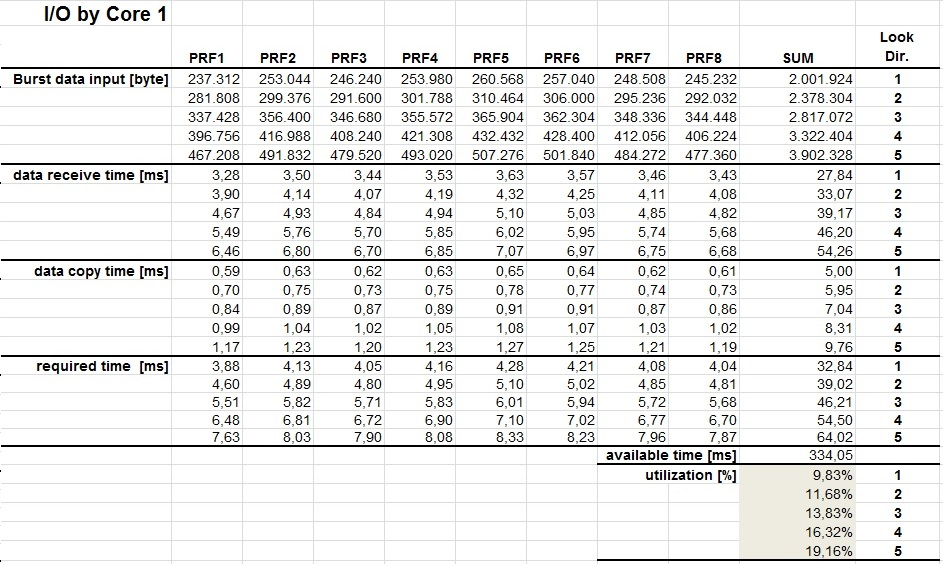
\includegraphics[width=150mm]{figures/aa_scheme1_cpu_util_1}
	\caption{Scheme-1, Core1 Utilization}
	\label{fig:existing_analysis:aa_scheme1_cpu_util1}
\end{figure}

\begin{align*}
	\label{aa:scheme1:core1:equ}
	Burst \enspace data \enspace input & = 64 pulses \enspace * \enspace 103 \frac{range gates}{pulse} \enspace * \enspace 9channel * 4\frac{byte}{sample}\\[0.3cm]
	& = 237,312 \enspace byte \\[0.3cm]
	Data \enspace receive \enspace time &= \frac{1}{19.5 \enspace * \enspace 10^{3} \enspace Hz} \enspace * \enspace 64 = 3.28 \enspace ms \\[0.3cm]
	Data \enspace copy \enspace time &= 237,312 byte \enspace * \enspace 2\frac{cycle}{byte} \enspace * \enspace 1.25\frac{ns}{cycle} = 0.59 \enspace ms \\[0.3cm]
	Required \enspace time &= 3.28ms + 0.59ms =  3.88ms\\[0.3cm]
	Available \enspace time &= 12 * min.dwelltime = 12*27.84ms = 334.05ms \stepcounter{equation}\tag{\theequation} 
\end{align*}

Core2 transfers the data from its buffer memory to storage memory to L2 cache and then performs Beamforming. The results of the processing are stored back to the core3's buffer memory in SDRAM. As shown in Figure \ref{fig:existing_analysis:aa_scheme1_cpu_util2}, maximum utilization of Core2 reaches upto 24\% of the available time. The burst data input and data copy time are the same as the Equation \ref{aa:scheme1:core1:equ}. Every beamformed sample occupies 8 byte of memory.
\begin{figure}[h!]
	\centering
	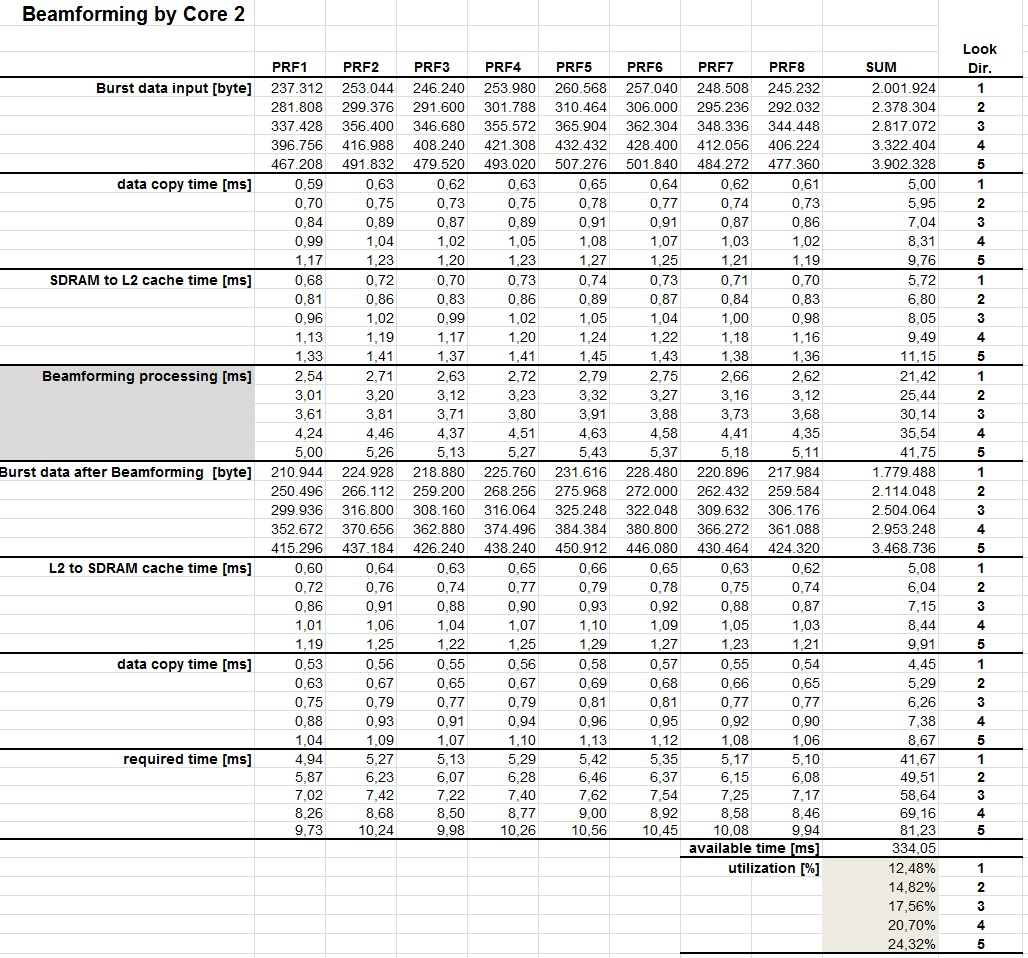
\includegraphics[width=150mm]{figures/aa_scheme1_cpu_util_2}
	\caption{Scheme-1, Core2 Utilization}
	\label{fig:existing_analysis:aa_scheme1_cpu_util2}
\end{figure}

\begin{align*}
\label{aa:scheme1:core2:equ1}
	SDRAM \: to \: L2cache \: time &= 237,312 byte \, * \, 2.29\frac{cycle}{byte} \, * \, 1.25\frac{ns}{cycle} = 0.68 \, ms \\[0.3cm]
	Beamforming \: processing &= 3channel * 64pulses * 103 \frac{range gates}{pulse} * 79\frac{cycle}{8 element} \\[0.3cm] 
	&\qquad * 1.25\frac{ns}{cycle} * 1.3(OSoverhead) = 2.54ms\\[0.3cm]
	Beamformed \: data &= 4channel * 64pulses * 103 \frac{range gates}{pulse} *8\frac{byte}{sample} = 210,944byte \\[0.3cm]
	L2cache \: to \: SDRAM \: time &= 210,944 byte \, * \, 2.29\frac{cycle}{byte} \, * \, 1.25\frac{ns}{cycle} = 0.60 \, ms \\[0.3cm]
	Data \: copy \: time &= 210,944 byte \, * \, 2.2\frac{cycle}{byte} \, * \, 1.25\frac{ns}{cycle} = 0.53 \, ms \\[0.3cm]
	Required \: time &= 0.59ms + 0.68ms + 2.54ms + 0.60ms + 0.53ms = 4.94ms \stepcounter{equation}\tag{\theequation} 
\end{align*}

Core3 reads the data from its SDRAM partition and performs Pulse Compression. The results of the processing are stored back to the SDRAM. Taken from Figure \ref{fig:existing_analysis:aa_scheme1_cpu_util3}, maximum utilization of Core3 is 65\% of the available time. Time required to copy the input data and store back pulse compressed data are the same as the Equation \ref{aa:scheme1:core2:equ1}. The input data set [64 x 103] is zero padded to the next power of 2 [64 x 128] to perform 128-point convolution.
\begin{figure}[h!]
	\centering
	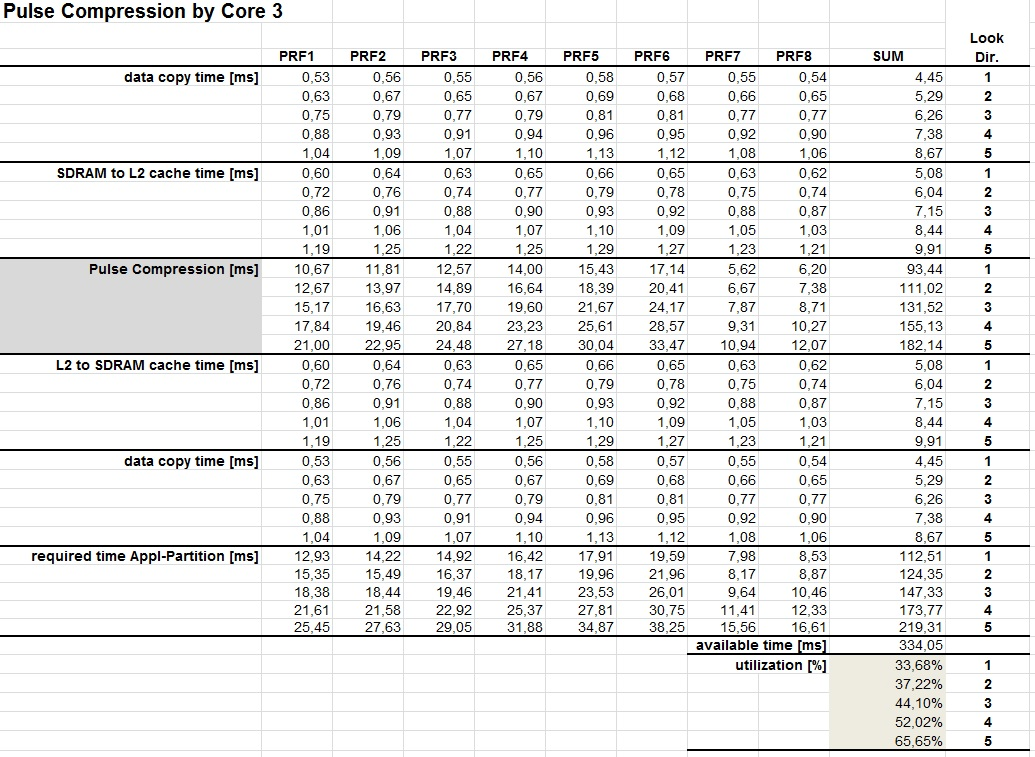
\includegraphics[width=160mm]{figures/aa_scheme1_cpu_util_3}
	\caption{Scheme-1, Core3 Utilization}
	\label{fig:existing_analysis:aa_scheme1_cpu_util3}
\end{figure}
\begin{align*}
	\label{aa:scheme1:core3:equ}
	Pulse \: compression &= \bigg(\#channel * \#pulses (CONV128 +  \# \frac{range gates}{pulse} * RMY50)\bigg)\\[0.3cm]  
	& \quad * \# \: cycle \: time * OSoverhead\\[0.3cm] 
	&= (4 * 64 (24100 + 103 * 15)) * 1.25 * 1.3 = 10.67ms   \stepcounter{equation}\tag{\theequation} 
\end{align*}

\FloatBarrier
Core4 gets the data from its SDRAM partition and performs FFT, CFAR, Correlation Processing. The results of the processing are stored back to the SDRAM. As mentioned in Figure \ref{fig:existing_analysis:aa_scheme1_cpu_util4}, maximum utilization of the Core4 is reaching 75\% of the available time.  Time required to copy the input data is same as the Equation \ref{aa:scheme1:core2:equ1}. FFT64 is chosen for Frequency Domain Transformation, as the corner turned data set size is [103 x 64].
\begin{figure}[h!]
	\centering
	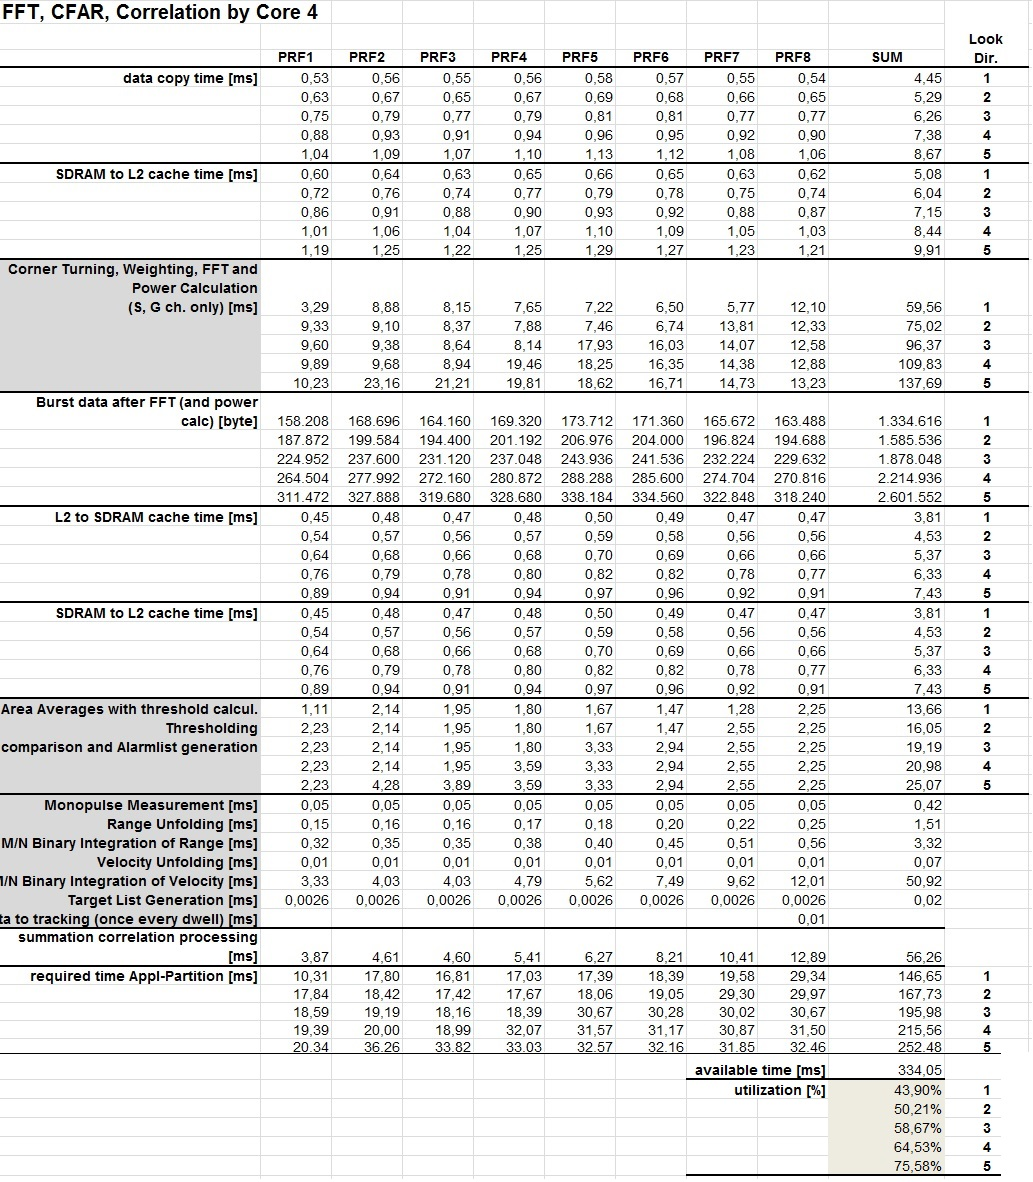
\includegraphics[width=150mm]{figures/aa_scheme1_cpu_util_4}
	\caption{Scheme-1, Core4 Utilization}
	\label{fig:existing_analysis:aa_scheme1_cpu_util4}
\end{figure}

\begin{align*}
	\label{aa:scheme1:core4:equ1}
	FDP \: time &= \bigg(4channel * (\#pulses * \# \frac{RG}{pulse} (COT50 + RMY50) + \# \frac{RG}{pulse} * FFT64) \\[0.3cm] 
	& \qquad + 2 * (\# \frac{range gates}{pulse} * 64 * MAG256)\bigg) * OSoverhead * cycle \, time \\[0.3cm]
	&= (4 * (64 * 103 (12 + 15) + 103 * 2550) + 2 * (103 * 64 * 20)) * 1.3 * 1.25ns \enspace \\[0.3cm]
	&= \enspace 3.29ms  \stepcounter{equation}\tag{\theequation} 
\end{align*}

After Frequency Domain Transformation and Magnitude Calculation, The Sum channel and Guard channel data have 4 byte per magnitude sample, Azimuth channel and Elevation channel data have 8 byte per complex sample.

\begin{align*}
	\label{aa:scheme1:core4:equ2}
		Data \: size \: after \: FDP &=  64pulses * 103 \frac{range gates}{pulse} ( 2 * 8 + 2 * 4) = 158,208 \: byte\\[0.25cm] 
		L2cache \: to \: SDRAM &= 158,208 byte \, * \, 2.29\frac{cycle}{byte} \, * \, 1.25\frac{ns}{cycle} = 0.45 \, ms \\[0.25cm]
		Average \: Calculation &= 2channel * 103 \frac{range gates}{pulse} * 64(FFTsize) * 20(AVG100) * 2 \\
		&=  527,360 \: cycle \\[0.25cm]
		Comparison &= 2channel * 103 \frac{range gates}{pulse} * 64(FFTsize) * 7(CMPR100) \\
		&= 92,288 \: cycle \\[0.25cm]
		Detection &= 1channel * 103 \frac{range gates}{pulse} * 64(FFTsize) * 10(DET100) \\
		&= 65,920 \: cycle \\[0.25cm]
		Time \: required &= (Average \, calculation + Comparison + Detection) \\
		& \qquad * OSoverhead * cycle \, time \\[0.25cm]
		&= (527,360 + 92,288 + 65,920) * 1.3 * 1.25ns = 1.1ms \stepcounter{equation}\tag{\theequation} 
\end{align*}

\begin{align*}
	\label{aa:scheme1:core4:equ3}
		Monopulse \: Measurement &= 2channel * \#\frac{alarms}{burst} * \#\frac{cycle}{alarm} * OSoverhead * cycle \: time \\
		&= 2 * 32 * 500 * 1.3 * 1.25ns = 0.05 \: ms \\
		Range \: Unfolding &= \bigg(RG_{max} * \#\frac{cycle}{rangegate} + \# Unfoldings * \#\frac{alarms}{burst} * \#cycle\bigg) \\
		& \qquad *OSoverhead * cycle \: time \\
		&= (987 * 30 + 10 * 32 * 200) * 1.3 * 1.25ns = 0.15 \: ms \\
		M/N \: Range \: Integration &= \bigg(\#RangeGates * \#\frac{cycle}{rangegate} + \#Unfoldings * \#\frac{alarms}{burst} \\
		&\qquad * \#\frac{cycle}{alarm}\bigg) * OSoverhead *cycle \: time \\
		&= (988 * 40 + 32 * 10 * 500) * 1.3 * 1.25ns = 0.32 \: ms \\
		Velocity \: Unfolding &= \bigg(\#Unfoldings * \#\frac{alarms}{burst} * \#\frac{cycle}{alarm}\bigg) \\
		& \qquad * OSoverhead * \#cycle \: time \\
		&= (8 * 32 * 30) * 1.3 * 1.25ns = 0.01 \: ms \\
		M/N \: Velocity \: Integration &= \bigg(\#\frac{alarms}{burst} * \#Unfoldings^{2} * \#bursts * \#\frac{cycle}{alarm}\bigg) \\
		& \qquad * OSoverhead * cycle \: time \\
		&= (32 * 10^{2} * 8 * 80) * 1.3 * 1.25ns =  3.33 \: ms \\
		Target \: List \: Generation &= \bigg(\#targets * \#\frac{cycle}{target}\bigg) * OSoverhead * cycle \: time \\
		&= (16 * 100) * 1.3 * 1.25ns = 0.0026 \: ms \\
		Correlation \: Processing[ms] &= 0.05 + 0.15 + 0.32 + 0.01 + 3.33 + 0.0026 = 3.87 \: ms \\
		Required \: time[ms] &= 0.53 + 0.60 + 3.29 + 0.45 + 0.45 + 0.11 + 3.87 = 10.31 \: ms \stepcounter{equation}\tag{\theequation}
\end{align*}


%%%%%%%%%%%%%%%%%%%%%%%%%
%%%%%  SSUB-SECTION   %%%
%%%%%%%%%%%%%%%%%%%%%%%%%
\subsubsection{Processing Latency}
\label{sss:scheme1:latency}
Processing Latency is the time between reception of a dwell and sending of processed result data. As listed in Table \ref{tbl:existing_analysis:aa_scheme1_latency}, processing latency between 333ms and 617ms is achieved depending on the look direction. In case of Active Electronically Scanned Array (AESA) Radar, processing latency influnces agility of the system. Beam steering is performed electronically in AESA Radar compared to the mechanical steering in conventional Radars. Dynamic carrier frequency and PRF characteristics of the AESA Radar makes it hard to be intercepted by Radar Warning Receiver. Derivation of Look direction-1's processing latency is explained below. 

\begin{align*}
	\label{aa:scheme1:latency}
		Processing \: latency &= IO + Beamforming + Pulse \: compression  + FFT,CFAR,Correlation \\
		&= 32.84 + 41.67 + 112.51 + 146.65 = 333.67 \: ms \\[0.3cm]
		\#Dwell \: latency &= \frac{processing \: latency}{dwell \: time} = \frac{333.67}{27.84} = 11.99 \stepcounter{equation}\tag{\theequation}
\end{align*}

\begin{table}[h!]
	\centering
	\begin{tabular}{|c|l|l|l|} 
	 \hline
	 \textbf{Look direction} & \textbf{Dwell time[ms]} & \textbf{Latency[ms]} & \textbf{\#Dwell latency} \\
	 \hline
	 1 & 27.84 & 333.67 & 11.99 \\ \hline
	 2 & 33.07 & 380.61 & 11.51 \\ \hline
	 3 & 39.17 & 448.16 & 11.44 \\ \hline
	 4 & 46.20 & 513.00 & 11.10 \\ \hline
	 5 & 54.26 & 617.05 & 11.37 \\ \hline
	\end{tabular}
	\caption{Scheme-1, A/A Mode Processing Latency}
	\label{tbl:existing_analysis:aa_scheme1_latency}
\end{table}

%%%%%%%%%%%%%%%%%%%%%%%%%
%%%%%  SSUB-SECTION   %%%
%%%%%%%%%%%%%%%%%%%%%%%%%
\subsubsection{Memory Utilization}
\label{sec:scheme1:mem_util}
Each CPU has 4GiB of externally connected SDRAM. It is assumed that 3GiB are allocated for OS, storing executable code, etc. 1GiB are available for the actual data processing. Input and output data size for the cores are explained in each core's CPU utilization section. Figure \ref{fig:existing_analysis:aa_scheme1_mem_util} shows that 7\% of the available capacity is sufficient for A/A Mode processing.

\begin{figure}[h!]
	\centering
	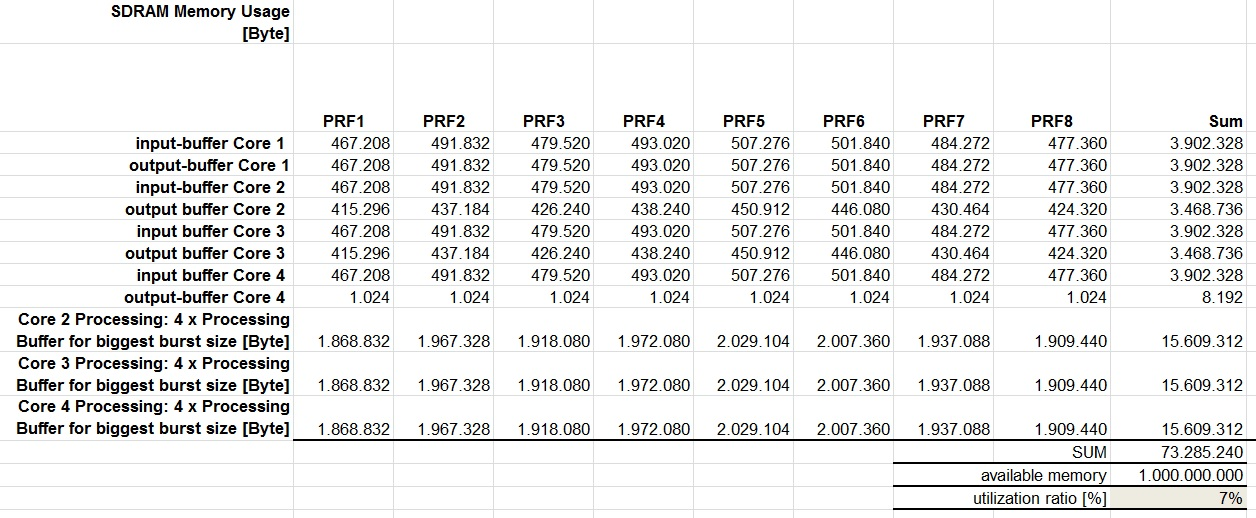
\includegraphics[width=160mm]{figures/aa_scheme1_mem_util}
	\caption{Scheme-1, Memory Utilization}
	\label{fig:existing_analysis:aa_scheme1_mem_util}
\end{figure}

%%%%%%%%%%%%%%%%%%%%%%%%%
%%%%%  SSUB-SECTION   %%%
%%%%%%%%%%%%%%%%%%%%%%%%%
\subsubsection{Interface Utilization}
\label{sec:scheme1:aa_interface_util}
Interfaces are the data routing paths in the Radar processor. Nominal bandwidth of 100MiB/s data rate is assumed for the interfaces. The DGPMs are identical, thus only one DGPM's utilization is listed here. As calculated in Figure \ref{fig:existing_analysis:aa_scheme1_interface_util}, peak interface utilization is inferred as 72\%.
\begin{figure}[h!]
	\centering
	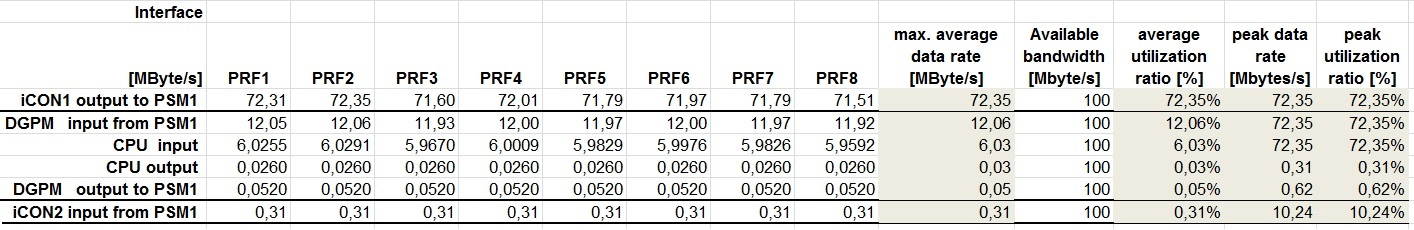
\includegraphics[width=160mm]{figures/aa_scheme1_interface_util}
	\caption{Scheme-1, Interface Utilization}
	\label{fig:existing_analysis:aa_scheme1_interface_util}
\end{figure}

\begin{align*}
	\label{equ:aa:scheme1:interface_util}
	iCON1 \: output \: to \: PSM1 &= \#\frac{byte}{sample} * \#channel * range \: gate * frequency \\
	&= 4 * 9 * 103 * 19.5kHz = 72.31 \: MB/s \\
	DGPM \: input \: from \: PSM &= \frac{data \: rate}{\#DGPMs} = \frac{72.31}{6} = 12.05 \: MB/s \\[0.3cm]
	CPU \: input &= \frac{DGPM \: data \: rate}{\#CPUs} = \frac{12.05}{2} = 6.02 \: MB/s \\[0.3cm]
	DGPM \: output \: to \: PSM &= \frac{data \: rate}{\#DGPMs} = \frac{0.31}{6} = 0.0526 \: MB/s \\[0.3cm]
	CPU \: output &= \frac{DGPM \: output}{\#CPUs} = \frac{0.0526}{2} = 0.026 \: MB/s \stepcounter{equation}\tag{\theequation}
\end{align*}
\FloatBarrier

\subsubsection{Summary}
The CPUs in the DGPM are physically separated for A/A Mode and A/G Mode; accordingly the results will not change if the Radar processor is performing both the modes simultaneously. Space partitioning has 12x dwell latency, utilizing 7\% of the available memory, 72\% of the interface and the following CPU utilization factors.

\begin{table}[h!]
	\centering
	\begin{tabular}{|l|l|l|l|l|} 
	 \hline
	& \textbf{Core1} & \textbf{Core2} & \textbf{Core3} & \textbf{Core4} \\ \hline
	\textbf{Utilization} & 19.16\% & 24.32\% & 65.65\% & 75.58\% \\ \hline
	\end{tabular}
	\caption{Scheme-1, CPU Utilization}
\end{table}



\clearpage
%%%%%%%%%%%%%%%%%%%%%%%%%%%%%%%%%%%%%
%%%%%%%%%%%%%%%%%%%%%%%%%%%%%%%%%%%%%
%%%%%%%%%%%%   SECTION   %%%%%%%%%%%%
%%%%%%%%%%%%%%%%%%%%%%%%%%%%%%%%%%%%%
%%%%%%%%%%%%%%%%%%%%%%%%%%%%%%%%%%%%%
\section{Scheme 2 - Time Partitioning}
\label{sec:scheme2}
This section explains the formulas and calculations in the excel document provided by Airbus DS. Every CPU runs both the A/A mode and A/G mode application concurrently. CPU time and resources are shared for both the applications. Memory is partitioned for each mode to provide segregation. This analysis assumes
\begin{compactitem}
	\item All the four cores of a CPU can access SDRAM without interfering each other.
	\item L2 cache is statically partitioned at compile time, partition values are stated in Figure \ref{fig:existing_analysis:scheme2_partition_values}.
	\item Partition change time is 0.5ms. 
\end{compactitem} 

Figure \ref{fig:existing_analysis:scheme2_partition} shows the time partitioning of a CPU. Each application has to complete processing and suspend itself before the time slice expires. Otherwise a "deadline miss exception" is triggered.

\begin{figure}[h!]
	\centering
	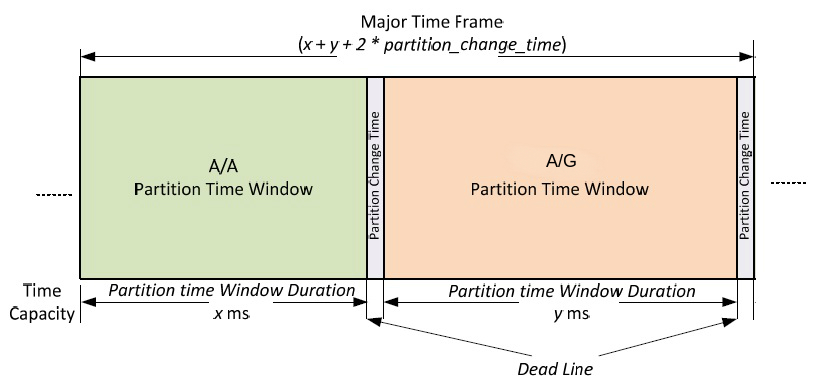
\includegraphics[height=55mm]{figures/scheme2_partition}
	\caption{Scheme-2, Time Partition}
	\label{fig:existing_analysis:scheme2_partition}
\end{figure}

A/A data and A/G data are distributed by iCON1 to PSM1 and PSM2 respectively. Processed A/A data are transferred to iCON2 through PSM1. Partially processed A/G results from CPU1...CPU20 are transfered to CPU21...CPU24, where final A/G processing is carried out, followed by the results of the A/G processing are sent via PSM2 and iCON2 to a display.

\begin{figure}[h!]
	\centering
	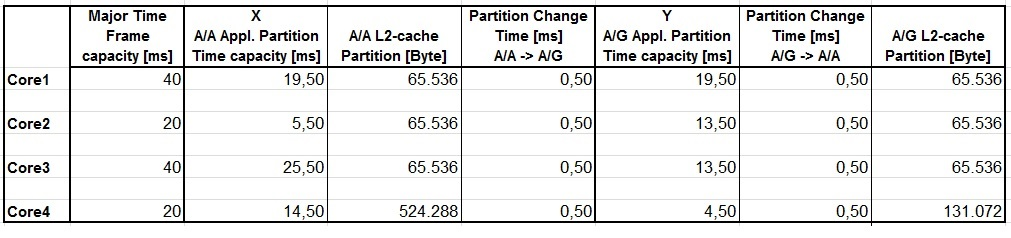
\includegraphics[width=150mm]{figures/scheme2_partition_values}
	\caption{Scheme-2, Values for Time Partition}
	\label{fig:existing_analysis:scheme2_partition_values}
\end{figure}

\begin{figure}[h!]
	\centering
	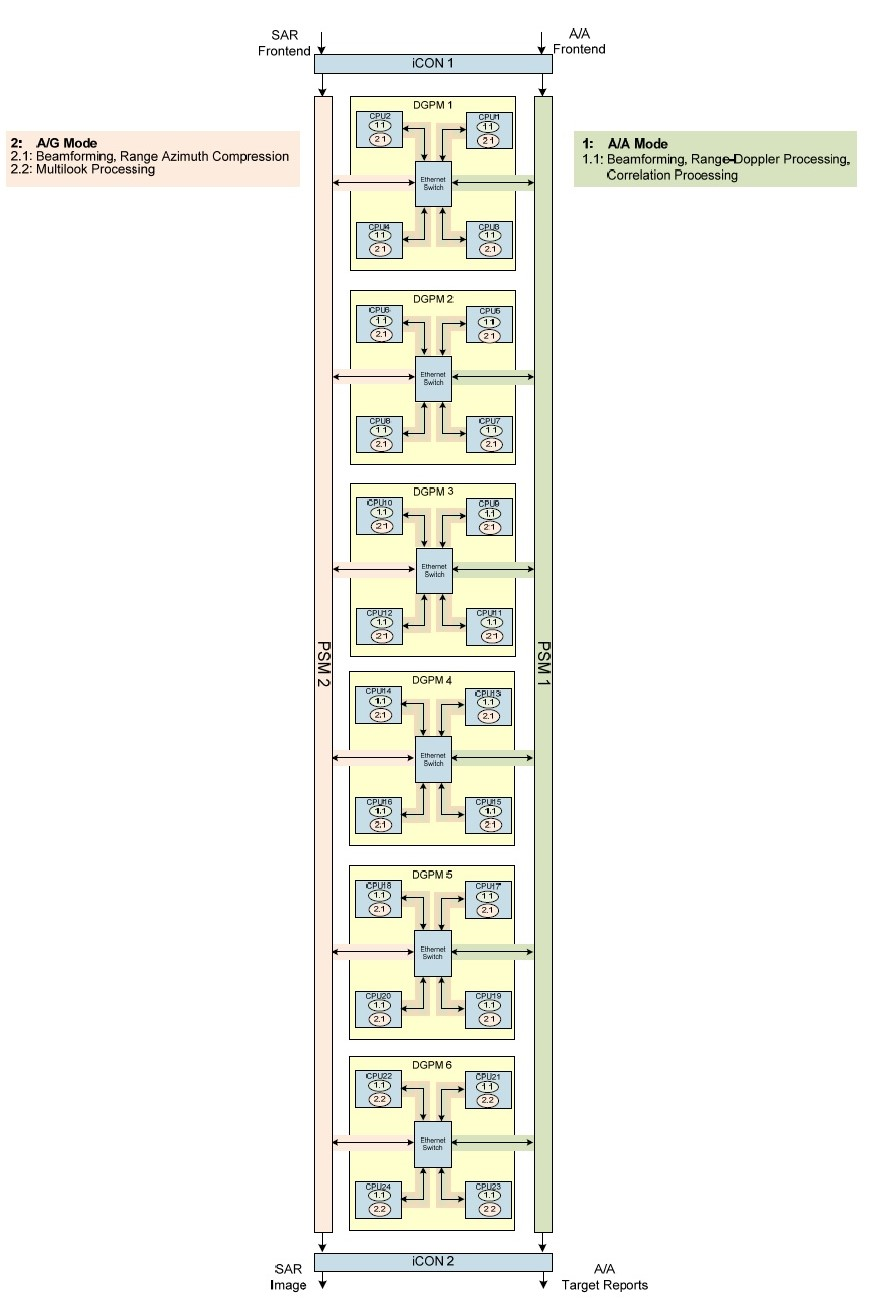
\includegraphics[width=160mm, height=220mm]{figures/scheme2_mode_mapping}
	\caption{Scheme-2, Mode Mapping}
	\label{fig:existing_analysis:scheme2_mode_mapping}
\end{figure}
\clearpage

\subsection{A/A Mode Results}
\label{ss:scheme2:aa}
A/A Mode configuration is similar to the configuration discussed in Scheme-1, (see Chapter \ref{ss:scheme1:aa}) except that the data is distributed to 24 CPUs. There may be some additional time slots required to fit the processing into the allotted time slice. For instance, 33 time slots would provide sufficient time to complete a certain processing having 65536 loop counts. Therefore 1985 loops could be processed in each time slot. An additional 34$^{th}$ time slot would be required to execute the remaining 31 loops. This is called Time Slot Adjustment. Calculations are same as Scheme-1 and hence details of the cores processing time are not shown for simplicity.

\subsubsection{CPU Utilization}
\label{sss:scheme2:cpu_util}
Available time is 24x shortest dwell time. Since the core is time sliced, effective available time is reduced by the factor of time slice and the processing latency is increased by the same factor. Table \ref{tbl:existing_analysis:aa_scheme2_cpu_util} lists the peak utilization values of each core.

\begin{table}[h!]
	\centering
	\begin{tabular}{|l|l|l|l|l|} 
	 \hline
	 & \textbf{Core1} & \textbf{Core2} & \textbf{Core3} & \textbf{Core4} \\ \hline
	 \textbf{Core Utilization} & 25\% & 53\% & 71\% & 63\% \\ \hline
	\end{tabular}
	\caption{Scheme-2, CPU Utilization}
	\label{tbl:existing_analysis:aa_scheme2_cpu_util}
\end{table}

\subsubsection{Processing Latency}
\label{sss:scheme2:latency}
Processing latency is higher than Scheme-1 because a core gets approximately half of the available time for A/A Mode processing. Processing latency between 640ms and 1100ms is achieved depending on the look direction, which is also listed in Table \ref{tbl:existing_analysis:aa_scheme2_latency}.

\begin{table}[h!]
	\centering
	\begin{tabular}{|c|l|l|l|} 
	 \hline
	 \textbf{Look direction} & \textbf{Dwell time[ms]} & \textbf{Latency[ms]} & \textbf{\#Dwell latency} \\
	 \hline
	 1 & 27.84 & 640 & 22.99 \\ \hline
	 2 & 33.07 & 700 & 21.17 \\ \hline
	 3 & 39.17 & 820 & 20.93 \\ \hline
	 4 & 46.20 & 880.00 & 19.05 \\ \hline
	 5 & 54.26 & 1100 & 20.27 \\ \hline
	\end{tabular}
	\caption{Scheme-2, A/A Mode Processing Latency}
	\label{tbl:existing_analysis:aa_scheme2_latency}
\end{table}

\subsubsection{Memory Utilization}
\label{sss:scheme2:mem_util}
Each CPU has 4GiB of externally connected SDRAM. It is assumed that 3GiB are allocated for OS, storing executable code, etc, 1GiB are available for data processing. As seen in Figure \ref{fig:existing_analysis:scheme2_aa_mem_util}, peak memory utilization reaches upto 9\% of the available memory.

\begin{figure}[h!]
	\centering
	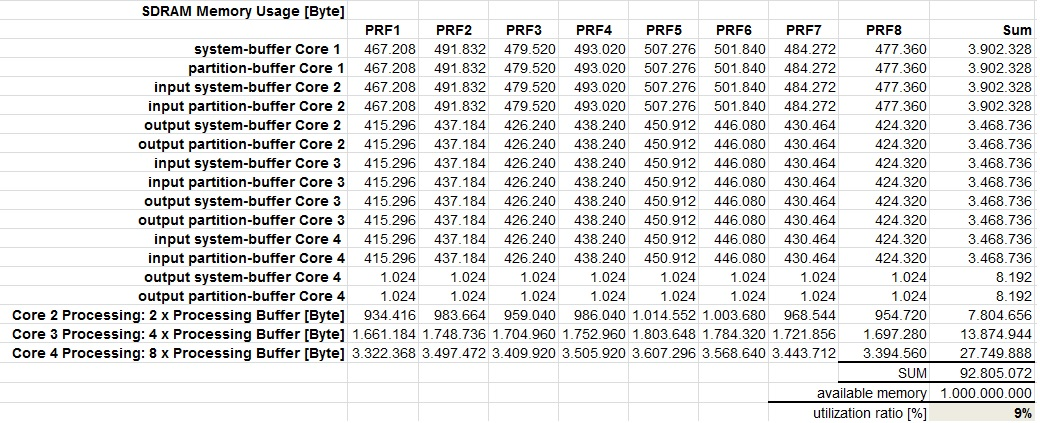
\includegraphics[width=160mm]{figures/scheme2_aa_mem_util}
	\caption{Scheme-2, Memory Utilization}
	\label{fig:existing_analysis:scheme2_aa_mem_util}
\end{figure}

\subsubsection{Interface Utilization}
\label{sss:scheme2:interface_util}
Data distribution scheme is the extended version of Scheme-1, hence the peak interface utilization remains same as 72\%.


\subsection{Summary}
\label{sss:scheme2:sar_summary}
The Time Partition configuration has 23x dwell time latency, utilizing 63\% of the CPU, 9\% of the memory and 72\% of the interface capability. Since every CPU is executing A/A mode processing as well as A/G mode processing, the combined results have to be taken into consideration to estimate peak values of the aforementioned profiling.

